% twocurv.tex
% May 2020
% association of follicle curvature and other skin and fleece traits with wrinkle differences in Merinos

\documentclass{article}


% Authors packages
\usepackage{graphicx,lscape,subfigure}
\usepackage{caption,rotating}
\usepackage{tikz}
\usepackage{bm,longtable}
\usepackage{textcomp}
\usepackage{url}


\begin{document}


\title{The two curvatures}
\author{Neville Jackson}
\date{31 Aug 2020}

\maketitle

\begin{abstract}

There is published evidence that follicles curve during follicle development and that the presence of hard collagen in the lower dermis at this time interferes with the developing follicle downgrowth causing follicles to grow in a curve.  
 There is also evidence of a strong association between fibre diameter, ortho/para cortical segmentation and general follicle size.

Conventional view of fibre curvature is that it is caused by differences in the ortho and para cortex. It is proposed that this may not be correct, and that both fibre curvature and microstructure difference between ortho and para cortex are caused by the fibre growing inside a curved follicle. 

It is proposed that follicle curvature has two components. Firstly, all follicles in all breeds of sheep are slightly curved and the degree of this component of curvature is related to fibre diameter. Secondly, if a sheep has the type of collagen that is associated with wrinkles, it also has some additional follicle curvature which is caused by collagen interfering with follicle development.

Some data and analyses are presented to support this 'two curvatures' hypothesis. In order for the two curvatures hypothesis to have a feasable mechanism it is necessary to assume that follicle curvature causes fibre curvature. We are able to present some data to support this  auxiliary assertion.
\end{abstract}


\section{Introduction}

Some time ago there was a wool industry which possessed a reasonable working definition of wool quality that was universally understood among producers, traders, and processors. They even went so far as to put a number on it, and to link it to spinning performance. Quality numbers  or 'Counts' ranged from 100's to 32's , the number referring to the number of hanks of yarn ( each 560 yards long)  which could be spun from 1 pound (0.454Kg) of clean wool, at the spinning limit. The concept is obviously tied to particular processing technologies. What is of interest here is the way quality number was assessed.  It was a visual appraisal of crimp frequency, with a correction for abnormal handle.

Then it was found that fibre fineness ( ie diameter) was a major determinant of spinning performance and softness or handle. There was a period of agonising over the relationship between crimp frequency and fibre diameter. We show some of these investigations in Figure~\ref{fig:crimpdiam} because they are relevant to our current arguments regarding curvature. 
%\documentclass{article}
%\usepackage{graphicx,subfigure}
%\usepackage{caption,rotating}
%\begin{document}

\begin{figure}[]
\centering
 \subfigure[Reviewed by Roberts and Dunlop]{
    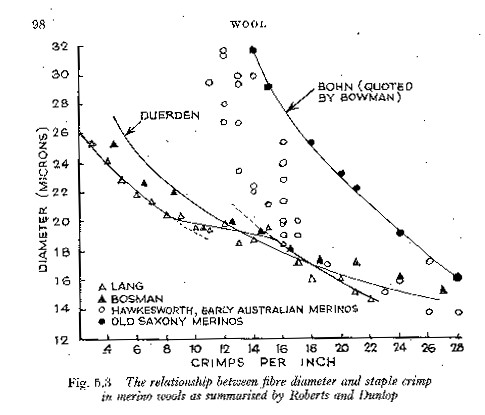
\includegraphics[scale=0.60]{cd1.jpg}
% \includegraphics[width=1.0\textwidth]{w479-2-rigid.jpg}
  }
 \subfigure[Roberts and Dunlop's own data from CSIRO Strain Trial]{
    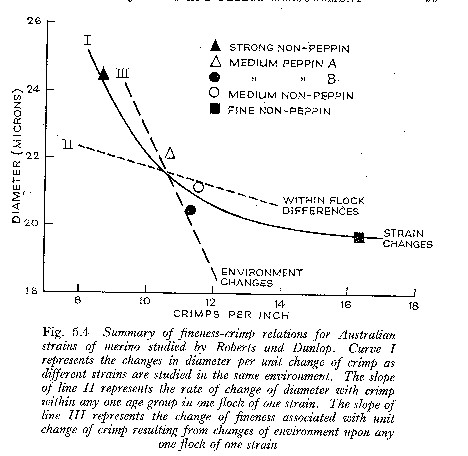
\includegraphics[scale=0.60]{cd2.jpg}
  }
  \caption{Crimp frequency fibre diameter relationships from Roberts and Dunlop(1957)~\cite{robe-1957}. Figures reproduced from Onions(1962)~\cite{onio-1962}}
\vfill
  \label{fig:crimpdiam}
\end{figure}

%\end{document}


Notice that the crimp/diameter relationship is quite steep at low crimp frequencies, but flattens out as one approaches the higher crimp frequencies of fine Merino wools. We are going to argue that the crimp/diameter relationship was historically quite satisfactory for non Merino wools, and that quality numbers as originally used for British sheep breeds were probably an adequate diameter indicator and therefore did indeed  relate to spinning performance. It is the Merino wools for which the quality number system breaks down. We will present new data making this clear; the above published material has an inadequate range, and is just what originally pointed us to the concept of crimp frequency relating to diameter for coarse wools but not for Merino.

Eventually measured fibre diameter replaced subjective quality numbers as a descriptor of wool sold in Australia, and elsewhere. The industry settled down to a period of about 20 years using fibre diameter alone. Then Paul Swan's thesis appeared defining fibre curvature and establishing a basic measurement method for fibre snippets and showing the importance of measurement conditions in ensuring that the fibre was relaxed for measurement (Swan(1993)~\cite{swan-1993}).  Fibre specification eventually became a dual parameter affair, with fibre diameter and fibre curvature both specified, but there is some doubt regarding the validity of the measurement conditions for fibre curvature with both Laserscan and OFDA measurement methods. 

In the middle of these market specification upheavals, sheep breeders also moved from quality numbers to fibre diameter, acknowledging that breeding of fine Merinos towards higher and higher quality numbers had not led to finer fibre diameters. Breeders also became interested, following the work of Nay(1966)~\cite{nay-1966}, in follicle curvature.  Follicle curvature was shown to be genetically correlated with staple crimp frequency, wrinkle score, and bulk compression measurement. The curvature of a follicle was always thought to be the same thing as the intrinsic curvature of a properly relaxed fibre, because it corresponded to the curvature with which the fibre emerged from the follicle. This was never proven. A formula converting follicle curvature scores to intrinsic radius of curvature was established by Jackson and Watts(2016)~\cite{jackson-2016}.

The focus of this document is on what causes follicles and fibres to be curved. There are two schools of thought on causation
\begin{description}
\item[classic view] fibres curve because of their internal structure. In sheep like fine Merinos with a bilateral ortho/para cortical structure, the paracortex is always on the inside of the curve. It is asserted that the paracortex contracts more during keratinization and thus causes the fibre to curve. The follicle passively follows what happens to the fibre. In coarser wooled sheep without bilateral cortical structure this is less clear, but Hynd et al. (2009)~\cite{hynd-2009} assert there is asymmetry in mitotic activity and keratinisation.
\item[follicle view] fibres curve because they form inside a curved follicle. The spatial environment in which the bulb cells differentiate influences their development leading to a different internal structure on the inside and outside of curves and a curved fibre shape.  The observed differences in internal fibre structure are just a side-effect of forming inside a curved follicle, and are not the cause of curvature. To find the cause of fibre curvature we have to look for what causes follicles to curve.  
\end{description}

This document takes the follicle view and attempts to uncover the causes of follicle curvature. It emerges that there is more than one causal factor, and that all are related to skin development, not to fibre structure.

\section{Causation and association}
Everyone u54nderstands that observing a correlation does not prove causation. So what experiments and analyses can one do to establish causation? There are several ways, and we list them
\begin{itemize}
\item Do a designed experiment. If the factors studied are the only difference between treatment groups, and there is proper randomization, then one can conclude the factors are responsible for the differences observed.
\item Establish a time sequence. If A occurs before B, then it is not possible for B to cause A.
\item Find a mechanism. If there is a feasable way in which A could cause B, then it is at least possible for A to cause B. Theories about how things work are very useful here.
\item  Strong correlation. There has to be some association observable between cause and effect. Observing association is a necessary step to establishing a cause, but it is not definitive.
\item Regression with chosen independent X values. This is like a designed factorial experiment. 
\item Repeatability. If a relation is causal it will always be present. 
\item Coherence. If a proposed causal relation fits in with other things known and generally accepted in an area, it is likely to be causal. If it is in disagreement, one has to be careful.
\end{itemize}
 
Behind most of these points is the concept of confounding. Designed experiments attempt to study factors in isolation. In the real world, especially in biology, we are often forced to study traits varying simultaneously.  Causal analysis in this situation  is difficult. One approach is to fit a model corresponding to one's theory of causation and to show that it is a good fit to the data. 


\section{Which comes first follicle or fibre curvature ?}
Evidence on the time sequence of follicle and fibre curvatures is not readily found. There is a photomicrograph in the classic study of Hardy and Lyne (1956)~\cite{hardy-1956} which shows developing follicles in vertical section before the fibre growth has commenced. This photomicrograph is important so we reproduce it here in Figure~\ref{fig:hardylyne}
%\documentclass{article}
%\usepackage{graphicx,subfigure}
%\usepackage{caption,rotating}
%\begin{document}

\begin{figure}[]
\centering
 \subfigure[Plate I from Hardy and Lyne(1956)~\cite{(hardy-1956}]{
  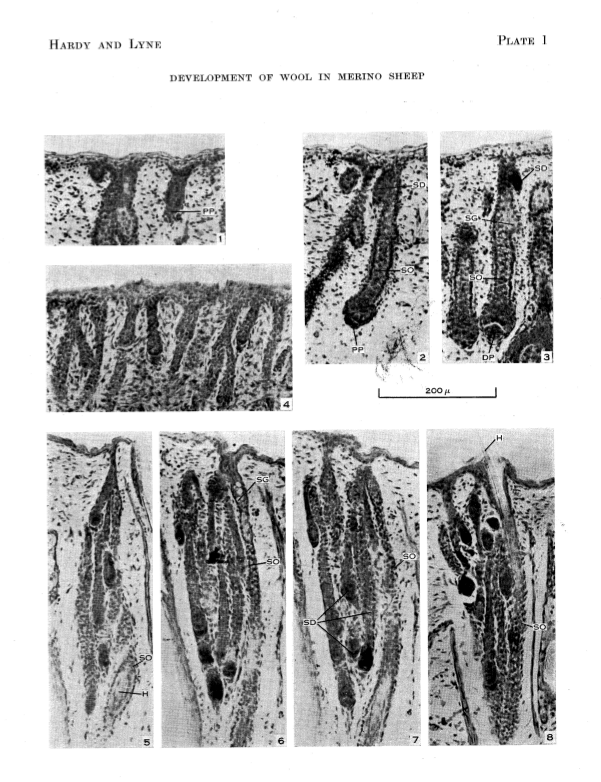
\includegraphics[width=1.0\textwidth]{HardyLyneplate1.png}
  }
 \subfigure[Caption from Hardy and Lyne(1956)~\cite{(hardy-1956}]{
  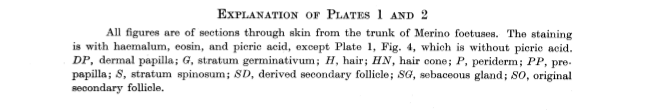
\includegraphics[width=1.0\textwidth]{HardyLynecaption.png}
  }

  \caption{ Follicles at some early stages of development}
\vfill
  \label{fig:hardylyne}
\end{figure}

%\end{document}


The fibre does not start to form before stage F4 and does not emerge from the follicle until stage F8. The first three photomicrographs, ie before stage F4, and the developing follicles show some curvature, especially in the second Figure. The fourth Figure shows branching follicles at day 102 .
This is hardly convincing evidence. The degree of curvature is slight. It is suspected that the Hardy and Lyne used a strong wooled Merino, as this would have been easier material to study vertical sections. 

\section{Follicle curvature and collagen}
As part of a study of association of collagen amount and type with wrinkle, it was observed that sheep in two groups chosen as wrinkle-free or wrinkled differed in amount and type of collagen in the lower dermis (Watts et al. (2020)~\cite{watts-2020}, but also differed in follicle curvature.  The group means for follicle curvature, and for fibre diameter, are shown in Table~\ref{tab:curv}
%\documentclass{article}
%\usepackage{lscape}
%\begin{document}

\begin{table}[htp]
\centering
\caption{Means for follicle curvature, fibre diameter and integrated collagen optical density for wrinkled and wrinkle-free groups of sheep}
\label{tab:curv}
\vspace{0.1in}
\begin{tabular}{|p{2.0in}|p{1.0in}|p{1.0in}|}  \hline
      & Wrinkle-free  &  Wrinkled  \\ 
\hline 
Follicle curvature (score 1-7) & 2.16 & 4.44 \\
Fibre diameter  (micron)    & 17.26 & 18.15 \\
Integrated collagen density (OD) & 280851 & 362991 \\
\hline

\end{tabular}
\end{table}

%\end{document}

The groups were chosen to differ in wrinkle. It has been proposed that the observed collagen difference is the cause of the difference in wrinkle (Watts et al. (2020)~\cite{watts-2020}). We are wondering whether the collagen difference is not also the cause of the difference in follicle curvature. 

What we propose is that presence of hard collagen in foetal skin during follicle development causes developing follicles to bend.  There is visual evidence of this occuring. Dreyer et al. (1983)~\cite{dreyer-1983} published a photomicrograph of Karakul sheep foetal skin in vertical section at 128 days. We reproduce it here in Figure~\ref{fig:dreyer}
%\documentclass{article}
%\usepackage{graphicx,subfigure}
%\usepackage{caption,rotating}
%\begin{document}

\begin{figure}[]
\centering
    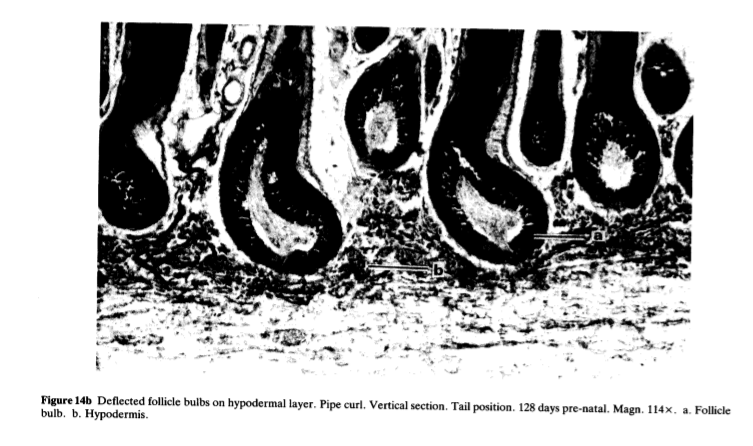
\includegraphics[scale=0.80]{dreyerp6.png}
  \caption{Photomicrograph of foetal skin from Dreyer et al. (1983)~\cite{dreyer-1983} showing follicle bulbs deflecting on contact with the collagen layer. Karakul sheep at 128 days}
\vfill
  \label{fig:dreyer}
\end{figure}

%\end{document}


We quote Dreyer et al
\begin{quote}
"The impression gained was that owing to the vigour of the follicle bulb, the constituent collagen fibres of the hypodermis were displaced in some cases, but no real piercing of that tissue took place. In other cases it would appear theat the follicle bulb and the papilla were undergoing some degree of flattening due to growth pressure on the barrier layer......This barrier effect could also explain the deflection of the bulb to any side as it reacts to the force exerted by downward growth"
\end{quote}
This clearly establishes that the dark stained collagen layer in Figure~\ref{fig:dreyer} acts as a barrier to downward growth of follicles.  If the follicles continue to grow, they must deflect sideways, and this will result in a curved follicle.

\section{Follicle curvature without collagen}
All follicles in non-Merino breeds of sheep have a slight degree of curvature, and their fibres or staples have a range of crimp frequencies less than one up to about 4 crimps per cm.  We may have to exclude Downs wool breeds, here because they have very curved and tangled follicles, and I suspect they have hard collagen induced follicle curvature like Merinos.

We have to consider what causes the curvature of follicles in sheep which do not have hard collagen? The first thing to note is it appears to be quite strongly related to fibre diameter. There are data supporting this in Figure~\ref{fig:crimpdiam} and in the subsection below.

Follicles have an inherant asymmetric design.  They have a thicker inner and outer root sheath on the ental side (side to which the muscle is attached in primary follicles), and this side is usually the outside of the curve. The bulb sometimes deflects toward this side.   Larger follicles tend to be less curved, hence the connection between curvature and fibre diameter, because larger follicles tend to grow larger fibres (Henderson(1964 a~\cite{henderson-1964}).

\subsection{Data supporting proposal that curvature relates to diameter in non-Merino breeds, but not in Merino}
The breed survey data of Carter(1968)~\cite{carter-1968} offer some support. There are no follicle or fibre curvature measurements, but there is crimp frequency and diameter. So we shall look at the crimp/diameter relationship  across breeds in particular comparing non-Merino with Merino data. Figure~\ref{fig:cartcrimpdia} plots breed means of fibre diameter against crimp frequency
%\documentclass{article}
%\usepackage{graphicx,subfigure}
%\usepackage{caption,rotating}
%\begin{document}

\begin{figure}[]
\centering
    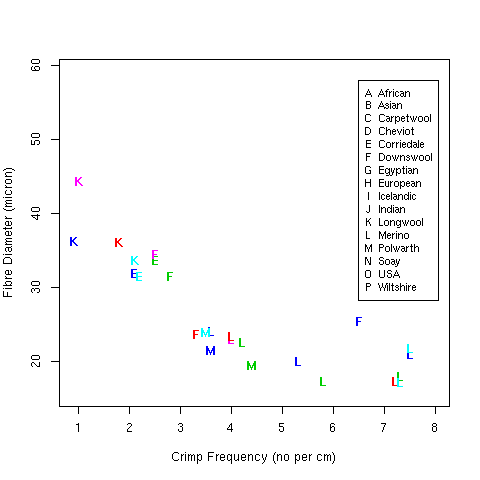
\includegraphics[scale=0.80]{cartercrimpdia.png}
  \caption{Crimp frequency fibre and diameter breed means from Carter(1968)~\cite{carter-1968}. Each point is mean of about 20 sheep from one flock representing a breed.}
\vfill
  \label{fig:cartcrimpdia}
\end{figure}

%\end{document}


There is a clear straight line relationship for crimp frequencies up to about 4 crimps per cm. In the Merino range ( 4 to 8 crimps per cm) there is no relationship at all, and there is one outlier Downs wool breed mean in that range. 

These data have limitations. There are not enough replicate points. We are using crimp frequency as a proxy for follicle curvature. Each point is a mean of about 20 sheep sampled from one flock representing the breed. The only positive is that it extends Figure~\ref{fig:crimpdiam} into the non-Merino breeds.

\section{Can we separate two causes for curvature?}
We are proposing that there is one follicle curvature, that all sheep have, that is related to fibre diameter and follicle size, and that there is a second follicle curvature that only Merinos have, that is caused by  presence of hard Type I collagen in the lower dermis.

Can we separate these {\em two curvatures} by analysing data?  I propose that we can use regression analysis to remove the diameter related part of follicle curvature variation, and then study the remaining variation ans see if it relates to collagen measurements.

\subsection{ Does diameter corrected follicle curvature relate to collagen measurements?}
The only available data that include collagen measurements, follicle curvature and fibre diameter are  from the collagen/wrinkle experiments reported by Watts et al. (2020)~\cite{watts-2020}. Taking all available data from this experiment, we look first at the regression of follicle curvature on mean fibre diameter. This is shown in Figure~\ref{fig:fcd}
%\documentclass{article}
%\usepackage{graphicx,subfigure}
%\usepackage{caption,rotating}
%\begin{document}

\begin{figure}[]
\centering
    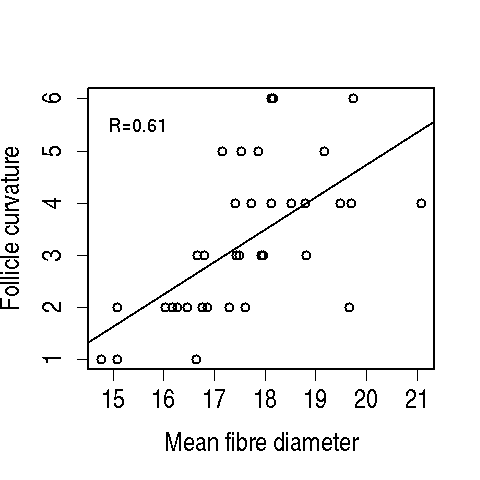
\includegraphics[scale=0.60]{fcd.png}
  \caption{Scatterplot of follicle curvature against mean fibre diameter for 35 sheep in the trial of Watts et al. (2020)~\cite{watts-2020}. Line is the fitted regression $(Fc ~ -7.68 + 0.62 * D)$, and correlation is shown as $R=0.61$.}
\vfill
  \label{fig:fcd}
\end{figure}

%\end{document}


Figure~\ref{fig:fcd} shows all data points, the regression line $(Fc ~  -7.68   + 0.621 * D)$ and the product moment correlation $(0.61)$. So part of the follicle curvature of these sheep is clearly diameter related.  The problem is this observed relationship is positive - the finer fibre diameter are {\em less} curved. According to our hypothesis (which is supported by the Carter(1968)~\cite{carter-1968} data), this relationship should be negative. 

THIS IS A SERIOUS ISSUE WHICH PUTS A QUESTION OVER THE HYPOTHESIS THAT PART OF FIOLLICLE CURVATURE IS DIAMETER RELATED. IT WAS THOUGHT THAT THE CARTER DATA IN Figure~\ref{fig:cartcrimpdia} SUPPORTED A DIAMETER-RELATED EFFECT ON CURVATURE. THAT MAY BE WRONG. WE NEED TO PAUSE AND DO 2 THINGS : 1. LOOK AT A LARGER DATA SET ( THE PRESENT SMALL DATA SET MAY BE BIASED FOR SOME REASON) and 2. THINK WHETHER OUR INTERPRETATION OF  Figure~\ref{fig:cartcrimpdia} IS CORRECT

THE FOLLOWING SECTION DETAILING AN ANALYSIS WHICH DEPENDS ON THE CURVATURE/DIAMETER RELATIONSHIP HAS BEEN PUT INTO TINY FONT, INDICATING THAT IT MAY BE WRONG OR INAPPROPRIATE. 

\begin{tiny}
 We remove this diameter related part of follicle curvature by computing the residuals for follicle curvature in Figure~\ref{fig:fcd}. We call these residuals $Fc | D$ (follicle curvature adjusted for diameter) and the computed residuals are shown as a histogram in Figure~\ref{fig:residhist} %\documentclass{article}
%\usepackage{graphicx,subfigure}
%\usepackage{caption,rotating}
%\begin{document}

\begin{figure}[]
\centering
    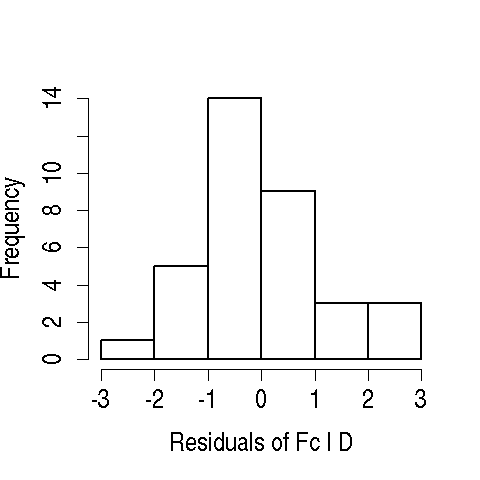
\includegraphics[scale=0.60]{fcdresidhist.png}
  \caption{Histogram histogram of residual variation in follicle curvature after adjusting for regression on mean fibre diameter}
\vfill
  \label{fig:residhist}
\end{figure}

%\end{document}


So this new variable $(Fc | D)$ has nearly as big a range as Fc and has a reasonable normal-looking distribution (this was tested with residual plots). The mean is zero because they are relativ to the mean curvature at a given diameter.

We can now look to see if this remaining variation in $Fc | D$ is related to collagen measurements. This relation is shown in Figure~\ref{fig:fcadjdxcoll}
%\documentclass{article}
%\usepackage{graphicx,subfigure}
%\usepackage{caption,rotating}
%\begin{document}

\begin{figure}[]
\centering
    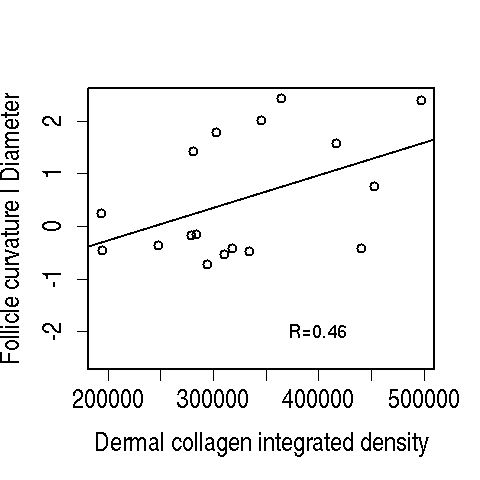
\includegraphics[scale=0.80]{fcadjdcoll.png}
  \caption{Scatterplot of follicle curvature adjusted for diameter against integtated dermal collagen optical density for 17 sheep in the trial of Watts et al. (2020)~\cite{watts-2020}. Line is the fitted regression $(Fc | D ~ -1.49 + 6.17e-06 * Collagen)$, and correlation is shown as $R=0.46$.}
\vfill
  \label{fig:fcadjdxcoll}
\end{figure}

%\end{document}


So Fc adjusted for D does related to collagen. There are only 17 points because this work was incomplete whn Jim Watts passed away. Only 17 sheep had Fc and D and Collagen measurements.

It is worth looking at the residuals from the fit in Figure~\ref{fig:fcadjdxcoll} to see how much variation in Fc still remains, unexplained by either D or Collagen.  We can do this by looking at variances. Variance of Fc was 1.91. Variance of Fc adjusted for D was 1.30. Variance of Fc adjusted for both D and Collagen was 1.04. So we have explained about half the variance of Fc using D and Collagen. The remaining half is probably measurement error, that is errors in scoring Fc and also errors in the D and Collagen measurements used for adjustment.

There are issues with this analysis
\begin{itemize}
\item the data are from a designed experiment in which sheep were chosen from 2 commercial flocks to represent extremes of wrinkle-free or wrinkled. The analysis did not fit Flock or SkinType effects. This would have removed most of the variation, especially in collagen density. 
\item the stepwise adjustment is not the conventional way of analysing effects of 2 variables on a third variate.  We do it stpewise first, so we can grasp what is happening. 
\item there is insufficient data
\item the diameter effect on follicle curvature is positive . We are proposing that in general it should ne negative.
\end{itemize}

\subsubsection{ Lets do it all again using multiple regression}
Just to show that the conclusions from the stepwise analysis of previous section are OK, we do a multiple regression of follicle curvature  on fibre diameter and collagen optical density. The result is summarised in Table~\ref{tab:mreg}
%\documentclass{article}
%\usepackage{lscape}
%\begin{document}

\begin{table}[htp]
\centering
\caption{Multiple regression of follicle cruvature $(Fc)$ on mean ffibre diameter$(D)$ and integrated collagen optical density $(C)$ for 17 sheep from Trial2 of Watts et al.(2020)~\cite{watts-2020}.}
\label{tab:mreg}
\vspace{0.1in}
\begin{tabular}{|p{0.8in}|p{0.8in}|p{0.8in}|p{0.8in}|p{0.8in}|}  \hline
      & Coefficient estimate & Std. Error & T value & Pr$(>|t|)$ \\
\hline 
 (Intercept) & -1.177e+01 & 4.678e+00 & -2.515  & 0.0247 * \\
 D           & 7.859e-01  & 2.894e-01 &  2.716  & 0.0167 * \\
 C           & 5.188e-06  & 3.589e-06 &  1.446  &  0.1703   \\
\hline

\end{tabular}
\end{table}

%\end{document}

The regression on $D$ is significant, that on $C$ is not, but it is at least positive. To interpret this multiple regression equation we need to convert the coefficients to standardized partial regression coefficients. THe standard deviations for $D$ and $C$ are $\sigma_{D} = 1.0645$ and $\sigma_{C} = 85844$. We multiply the coefficients in Table~\ref{tab:mreg} by these to get the standardised partial regression coefficients $\beta_{D} = 0.8366$ and $\beta_{C} = 0.4454$. The proportions of variance explained are therefore the squares of these $\beta's$ , ie .6998 and .1983. These sum to .8982, so we have explained 89\% of ther varaince of $Fc$ and the remainder $(1-.8982 = .1018)$ shows 10 percent of the varaince unexplained.

This is not exactly the same as the stepwise analysis of the previous section, and the reason is that more than 17 observations were used for the first step ( regression of $Fc$ on $D$). 

One can express the outcome of this multiple regression analysis as a path diagram (Wright(...)~\cite{wright-}). The path diagram is shown in Figure~\ref{fig:path}

% Graphic for TeX using PGF
% Title: /common/Dia/fc.dia
% Creator: Dia v0.97.3
% CreationDate: Thu Sep  3 20:48:08 2020
% For: nevj
% \usepackage{tikz}

%\documentclass{article}
%\usepackage{graphicx,lscape}
% \usepackage{tikz}
%\begin{document}
\begin{figure}[!h]
  \centering

% The following commands are not supported in PSTricks at present
% We define them conditionally, so when they are implemented,
% this pgf file will use them.
\ifx\du\undefined
  \newlength{\du}
\fi
\setlength{\du}{15\unitlength}
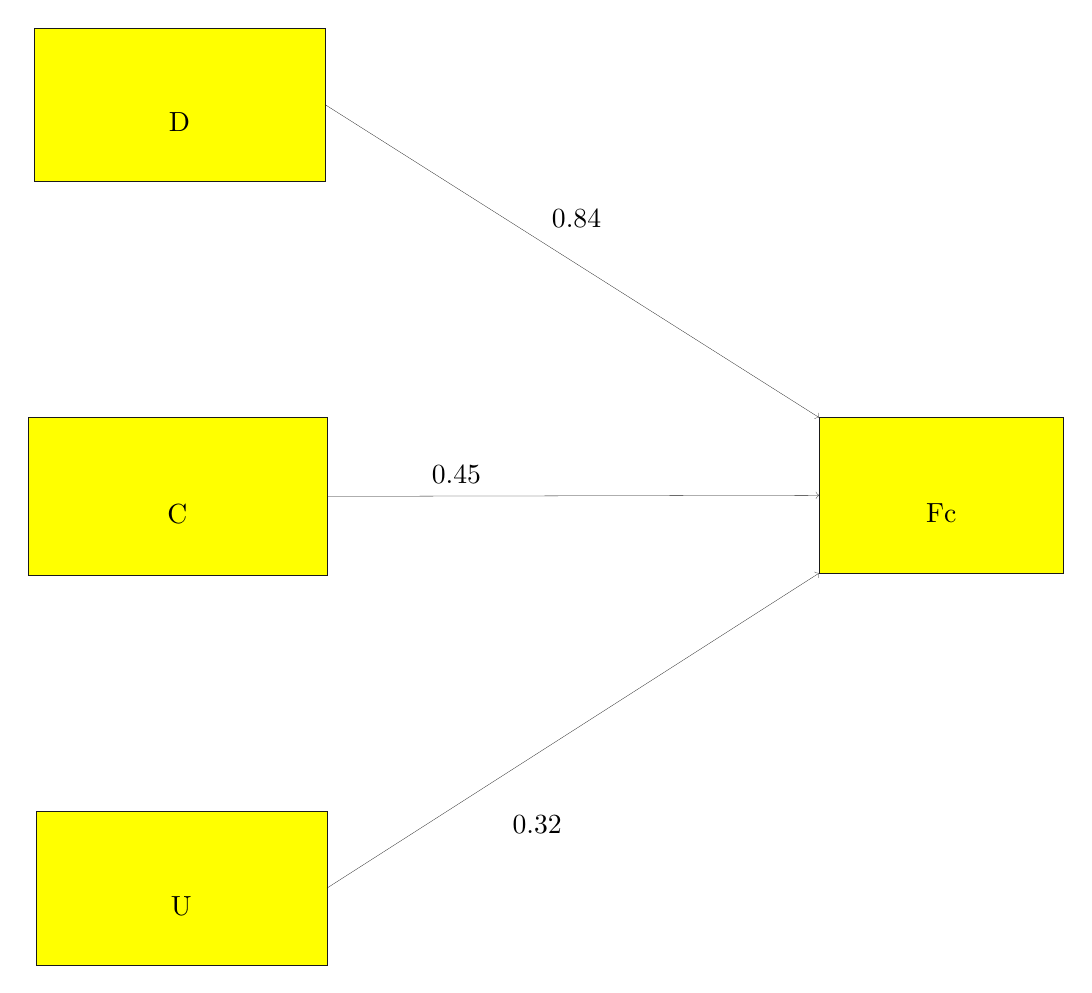
\begin{tikzpicture}
\pgftransformxscale{1.000000}
\pgftransformyscale{-1.000000}
\definecolor{dialinecolor}{rgb}{0.000000, 0.000000, 0.000000}
\pgfsetstrokecolor{dialinecolor}
\definecolor{dialinecolor}{rgb}{1.000000, 1.000000, 1.000000}
\pgfsetfillcolor{dialinecolor}
\pgfsetlinewidth{0.100000\du}
\pgfsetdash{}{0pt}
\pgfsetdash{}{0pt}
\pgfsetmiterjoin
\definecolor{dialinecolor}{rgb}{1.000000, 1.000000, 0.000000}
\pgfsetfillcolor{dialinecolor}
\fill (2.025000\du,2.050000\du)--(2.025000\du,4.000000\du)--(5.725000\du,4.000000\du)--(5.725000\du,2.050000\du)--cycle;
\definecolor{dialinecolor}{rgb}{0.101961, 0.101961, 0.101961}
\pgfsetstrokecolor{dialinecolor}
\draw (2.025000\du,2.050000\du)--(2.025000\du,4.000000\du)--(5.725000\du,4.000000\du)--(5.725000\du,2.050000\du)--cycle;
\pgfsetlinewidth{0.100000\du}
\pgfsetdash{}{0pt}
\pgfsetdash{}{0pt}
\pgfsetmiterjoin
\definecolor{dialinecolor}{rgb}{1.000000, 1.000000, 0.000000}
\pgfsetfillcolor{dialinecolor}
\fill (1.950000\du,7.000000\du)--(1.950000\du,9.000000\du)--(5.750000\du,9.000000\du)--(5.750000\du,7.000000\du)--cycle;
\definecolor{dialinecolor}{rgb}{0.101961, 0.101961, 0.101961}
\pgfsetstrokecolor{dialinecolor}
\draw (1.950000\du,7.000000\du)--(1.950000\du,9.000000\du)--(5.750000\du,9.000000\du)--(5.750000\du,7.000000\du)--cycle;
\pgfsetlinewidth{0.100000\du}
\pgfsetdash{}{0pt}
\pgfsetdash{}{0pt}
\pgfsetmiterjoin
\definecolor{dialinecolor}{rgb}{1.000000, 1.000000, 0.000000}
\pgfsetfillcolor{dialinecolor}
\fill (2.050000\du,12.000000\du)--(2.050000\du,13.950000\du)--(5.750000\du,13.950000\du)--(5.750000\du,12.000000\du)--cycle;
\definecolor{dialinecolor}{rgb}{0.101961, 0.101961, 0.101961}
\pgfsetstrokecolor{dialinecolor}
\draw (2.050000\du,12.000000\du)--(2.050000\du,13.950000\du)--(5.750000\du,13.950000\du)--(5.750000\du,12.000000\du)--cycle;
\pgfsetlinewidth{0.100000\du}
\pgfsetdash{}{0pt}
\pgfsetdash{}{0pt}
\pgfsetmiterjoin
\definecolor{dialinecolor}{rgb}{1.000000, 1.000000, 0.000000}
\pgfsetfillcolor{dialinecolor}
\fill (12.000000\du,7.000000\du)--(12.000000\du,8.975000\du)--(15.100000\du,8.975000\du)--(15.100000\du,7.000000\du)--cycle;
\definecolor{dialinecolor}{rgb}{0.101961, 0.101961, 0.101961}
\pgfsetstrokecolor{dialinecolor}
\draw (12.000000\du,7.000000\du)--(12.000000\du,8.975000\du)--(15.100000\du,8.975000\du)--(15.100000\du,7.000000\du)--cycle;
\pgfsetlinewidth{0.100000\du}
\pgfsetdash{}{0pt}
\pgfsetdash{}{0pt}
\pgfsetbuttcap
{
\definecolor{dialinecolor}{rgb}{0.101961, 0.101961, 0.101961}
\pgfsetfillcolor{dialinecolor}
% was here!!!
\pgfsetarrowsend{to}
\definecolor{dialinecolor}{rgb}{0.101961, 0.101961, 0.101961}
\pgfsetstrokecolor{dialinecolor}
\draw (5.725000\du,3.025000\du)--(12.000000\du,7.000000\du);
}
\pgfsetlinewidth{0.100000\du}
\pgfsetdash{}{0pt}
\pgfsetdash{}{0pt}
\pgfsetbuttcap
{
\definecolor{dialinecolor}{rgb}{0.101961, 0.101961, 0.101961}
\pgfsetfillcolor{dialinecolor}
% was here!!!
\pgfsetarrowsend{to}
\definecolor{dialinecolor}{rgb}{0.101961, 0.101961, 0.101961}
\pgfsetstrokecolor{dialinecolor}
\draw (5.750000\du,8.000000\du)--(12.000000\du,7.987500\du);
}
\pgfsetlinewidth{0.100000\du}
\pgfsetdash{}{0pt}
\pgfsetdash{}{0pt}
\pgfsetbuttcap
{
\definecolor{dialinecolor}{rgb}{0.101961, 0.101961, 0.101961}
\pgfsetfillcolor{dialinecolor}
% was here!!!
\pgfsetarrowsend{to}
\definecolor{dialinecolor}{rgb}{0.101961, 0.101961, 0.101961}
\pgfsetstrokecolor{dialinecolor}
\draw (5.750000\du,12.975000\du)--(12.000000\du,8.975000\du);
}
% setfont left to latex
\definecolor{dialinecolor}{rgb}{0.101961, 0.101961, 0.101961}
\pgfsetstrokecolor{dialinecolor}
\node[anchor=west] at (3.875000\du,3.025000\du){};
% setfont left to latex
\definecolor{dialinecolor}{rgb}{0.101961, 0.101961, 0.101961}
\pgfsetstrokecolor{dialinecolor}
\node at (3.875000\du,3.247500\du){D};
% setfont left to latex
\definecolor{dialinecolor}{rgb}{0.101961, 0.101961, 0.101961}
\pgfsetstrokecolor{dialinecolor}
\node at (3.850000\du,8.222500\du){C};
% setfont left to latex
\definecolor{dialinecolor}{rgb}{0.101961, 0.101961, 0.101961}
\pgfsetstrokecolor{dialinecolor}
\node at (3.900000\du,13.197500\du){U};
% setfont left to latex
\definecolor{dialinecolor}{rgb}{0.101961, 0.101961, 0.101961}
\pgfsetstrokecolor{dialinecolor}
\node at (13.550000\du,8.210000\du){Fc};
% setfont left to latex
\definecolor{dialinecolor}{rgb}{0.101961, 0.101961, 0.101961}
\pgfsetstrokecolor{dialinecolor}
\node[anchor=west] at (8.487500\du,4.475000\du){0.84};
% setfont left to latex
\definecolor{dialinecolor}{rgb}{0.101961, 0.101961, 0.101961}
\pgfsetstrokecolor{dialinecolor}
\node[anchor=west] at (13.550000\du,8.975000\du){};
% setfont left to latex
\definecolor{dialinecolor}{rgb}{0.101961, 0.101961, 0.101961}
\pgfsetstrokecolor{dialinecolor}
\node[anchor=west] at (6.962500\du,7.725000\du){0.45};
% setfont left to latex
\definecolor{dialinecolor}{rgb}{0.101961, 0.101961, 0.101961}
\pgfsetstrokecolor{dialinecolor}
\node[anchor=west] at (7.987500\du,11.775000\du){};
% setfont left to latex
\definecolor{dialinecolor}{rgb}{0.101961, 0.101961, 0.101961}
\pgfsetstrokecolor{dialinecolor}
\node[anchor=west] at (7.987500\du,12.175000\du){0.32};
\end{tikzpicture}
\caption{Path diagram expressing diameter $(D)$ related effects on follicle curvature, collagen $(C)$ related effeects on follicle curvature $(Fc)$, and other undefined effects $(U)$. The labels on each arrow are standardised partial regression coefficients. The square of each coefficient indicates prooprtion of variance explained. There may bo correlations among $(D.C.U)$ but these are not shown}
\label{fig:path}
\end{figure}
%\end{document}

Figure~\ref{fig:path} is just an illustration of how the present data supports the hypothesis that there are diameter-related and collagen-related parts of follicle curvature. 

The big issue is that the standardized partial regression for diameter is positive, where we are proposing that it should be negative if all other effects are averaged out properly.  We therefore have to shelve this analysis, and try to do something on a larger and more typical Merino dataset.

\end{tiny}

\subsection{Follicle curvature and fibre diameter in Merinos}
\label{sec:pubcor}
The relationship of follicle curvature with fibre diameter can be checked from published estimates. Table~\ref{tab:fcd} presents published estimates of phenotypic, genetic and environmental correlation. Standard errors can be obtained from the sources, they are a distraction here.
%\documentclass{article}
%\usepackage{lscape}
%\begin{document}

\begin{table}[htp]
\centering
\caption{Published estimates of phenotypic, genetic and environmental correlation between follicle curvature score and mean fibre diameter}
\label{tab:fcd}
\vspace{0.1in}
\begin{tabular}{|p{2.0in}|p{1.0in}|p{1.0in}|p{1.0in}|}  \hline
 Reference  & Phenotypic correlation  &  Genetic correlation & Environmeltal correlation  \\ 
\hline 
Jackson Nay and Turner (1975)~\cite{jackson-1975} & 0.26 & 0.32 & 0.22 \\
Jackson(2017)~\cite{jackson-2017a}    & 0.35 & 0.13 & 0.62 \\
\hline

\end{tabular}
\end{table}

%\end{document}

The correlations are all positive. So we conclude the small dataset above is not atypical or biased. Follicle curvature really does have a positive relationship with mean fibrte diameter in Merino sheep.

Now what about diameters of primary and secondary fibres? Estimates of correlations of follicle curvature with Dp and Ds are given in Table~\ref{tab:fcdpds}
%\documentclass{article}
%\usepackage{lscape}
%\begin{document}

\begin{table}[htp]
\centering
\caption{Estimates of phenotypic, genetic and environmental correlation between follicle curvature score and mean fibre diameter of primary and secondary fibres (Jackson(2017)~\cite{jackson-2017a}}
\label{tab:fcdpds}
\vspace{0.1in}
\begin{tabular}{|p{2.0in}|p{1.0in}|p{1.0in}|p{1.0in}|}  \hline
 Traits  & Phenotypic correlation  &  Genetic correlation & Environmeltal correlation  \\ 
\hline 
Fc x Dp & -0.02 & -0.32 & 0.25 \\
Fc x Ds    & 0.33 & 0.72 & 0.03 \\
\hline

\end{tabular}
\end{table}

%\end{document}

This is more complicated. At least at the genetic level, follicle curvature is negatively correlated with Dp, but positively correlated with Ds. So our hypothesis of a D related curvature component works for primary fibres, but not for secondary fibres. That partly explains Carter's data shown in Figure~\ref{fig:cartcrimpdia} - In the non-Merino breeds where there is this negative crimp frequency x diameter relation, primary fibres are a much larger proportion of the fibre population. It may be that the negative relationship obtained for primary fibres also applies to So ( secondary original fibres), because , as with primary fibres, So fibres form at initiation sites. P and So fibres would be all the fibres in non-Merino breeds. 

It is conceivable that follicle curvature in Sd fibres is different, and that would explain why Merinos have a different Fc x D relationship. One way in which curvature of Sd follicles could be different is that Sd follicles are formed at the same time as collagen is formed , at around 100 days of gestation. So collagen may only interfere with the curvature of Sd fibres.  

\subsubsection{Does Dp corrected follicle curvature relate to collagen measurements?}
We attempt to repeat the above rejected analysis, using Dp to remove the follicle size effect on follicle curvature, instead of D.

Table~\ref{fig:fcdp} shows follicle curvature plotted against primary fibre diameter for the data from the collagen/wrinkle experiment of Watts et al.(2020)~\cite{watts-2020}.
%\documentclass{article}
%\usepackage{graphicx,subfigure}
%\usepackage{caption,rotating}
%\begin{document}

\begin{figure}[]
\centering
    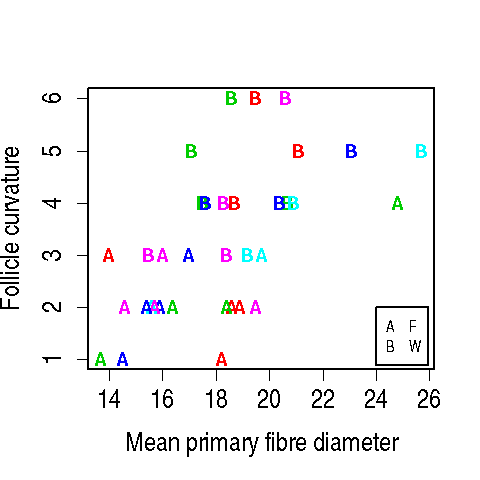
\includegraphics[scale=0.60]{fcdp.png}
  \caption{Scatterplot of follicle curvature against mean primary fibre diameter for 35 sheep in the trial of Watts et al. (2020)~\cite{watts-2020}. The correlation is  $R=0.59$.}
\vfill
  \label{fig:fcdp}
\end{figure}

%\end{document}


The correlation is positive, and almost identical to the correlation of Fc x D. So this dataset is different from the large datasets from which published estimates of correlation were reported in Section~\ref{sec:pubcor}.

We can not proceed with the use of Dp to adjust Fc in this small dataset. 

\subsubsection{Can we do the stepwise analysis in reverse order, adjusting follicle curvature first for collagen?}
This is a last ditch desperate approach. We are trying to prove that collagen affects follicle curvature. The diameter effect on follicle curvature is the nuisance relationship which should be adjusted out. But that is proving difficeult,  so we can try adjusting out the collagen effect on curvature, and see what variation remains.

Figure~\ref{fig:fccoll} shows the plot of follicle curvature against collagen measurement. 
%\documentclass{article}
%\usepackage{graphicx,subfigure}
%\usepackage{caption,rotating}
%\begin{document}

\begin{figure}[]
\centering
    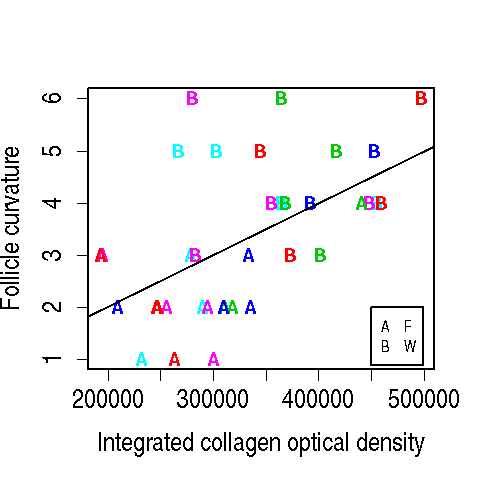
\includegraphics[scale=0.60]{fccoll.png}
  \caption{Scatterplot of follicle curvature against integrated collagen optical density for 35 sheep in the trial of Watts et al. (2020)~\cite{watts-2020}. Line is the fitted regression $(Fc ~ 0.96 + 0.00584 * C)$, and correlation is  $R=0.55$.The point labels (A,B) represent wrinkle-free (F) and wrinkled (W) sheep respectively. }
\vfill
  \label{fig:fccoll}
\end{figure}

%\end{document}


The correlation is positive (0.55), as expected.  The regression line was $Fc ~ 0.9601 + 5.843e-03 * C $.  



\subsection{ Follicle curvature analysis in a large Merino dataset}
 There are plenty of large follicle curvature datasets on Merinos. The problem is none of them have collagen measurements. What we propose to do is to use wrinkle score as a {\em proxy} for collagen. Either raw wrinkle score, or perhaps wrinkle score adjusted for S/P ratio (this would hopefully represent the part of wrinkle reflecting collagen amount and type).

\section{Mechanisms}


\bibliographystyle{plain}
\bibliography{twocurv}

\end{document}
